
\documentclass[letterpaper,hide notes,xcolor={table,svgnames},pdftex,10pt]{beamer}
\def\showexamples{t}


%\usepackage[svgnames]{xcolor}

%% Demo talk
%\documentclass[letterpaper,notes=show]{beamer}

\usecolortheme{crane}
\setbeamertemplate{navigation symbols}{}

\usetheme{MyPittsburgh}
%\usetheme{Frankfurt}

%\usepackage{tipa}

\usepackage{hyperref}
\usepackage{graphicx,xspace}
\usepackage[normalem]{ulem}
\usepackage{multicol}

\newcommand\SF[1]{$\bigstar$\footnote{SF: #1}}

\usepackage[default]{sourcesanspro}
\usepackage[T1]{fontenc}

\newcounter{tmpnumSlide}
\newcounter{tmpnumNote}

% old question code
%\newcommand\question[1]{{$\bigstar$ \small \onlySlide{2}{#1}}}
% \newcommand\nquestion[1]{\ifdefined \presentationonly \textcircled{?} \fi \note{\par{\Large \textbf{?}} #1}}
% \newcommand\nanswer[1]{\note{\par{\Large \textbf{A}} #1}}


 \newcommand\mnote[1]{%
   \addtocounter{tmpnumSlide}{1}
   \ifdefined\showcues {~\tiny\fbox{\arabic{tmpnumSlide}}}\fi
   \note{\setlength{\parskip}{1ex}\addtocounter{tmpnumNote}{1}\textbf{\Large \arabic{tmpnumNote}:} {#1\par}}}

\newcommand\mmnote[1]{\note{\setlength{\parskip}{1ex}#1\par}}

%\newcommand\mnote[2][]{\ifdefined\handoutwithnotes {~\tiny\fbox{#1}}\fi
% \note{\setlength{\parskip}{1ex}\textbf{\Large #1:} #2\par}}

%\newcommand\mnote[2][]{{\tiny\fbox{#1}} \note{\setlength{\parskip}{1ex}\textbf{\Large #1:} #2\par}}

\newcommand\mquestion[2]{{~\color{red}\fbox{?}}\note{\setlength{\parskip}{1ex}\par{\Large \textbf{?}} #1} \note{\setlength{\parskip}{1ex}\par{\Large \textbf{A}} #2\par}\ifdefined \presentationonly \pause \fi}

\newcommand\blackboard[1]{%
\ifdefined   \showblackboard
  {#1}
  \else {\begin{center} \fbox{\colorbox{blue!30}{%
         \begin{minipage}{.95\linewidth}%
           \hspace{\stretch{1}} Some space intentionally left blank; done at the blackboard.%
         \end{minipage}}}\end{center}}%
         \fi%
}



%\newcommand\q{\tikz \node[thick,color=black,shape=circle]{?};}
%\newcommand\q{\ifdefined \presentationonly \textcircled{?} \fi}

\usepackage{listings}
\lstset{%
  keywordstyle=\bfseries,
  aboveskip=15pt,
  belowskip=15pt,
  captionpos=b,
  identifierstyle=\ttfamily,
  escapeinside={(*@}{@*)},
  stringstyle=\ttfamiliy,
  frame=lines,
  numbers=left, basicstyle=\scriptsize, numberstyle=\tiny, stepnumber=0, numbersep=2pt}

\usepackage{siunitx}
\newcommand\sius[1]{\num[group-separator = {,}]{#1}\si{\micro\second}}
\newcommand\sims[1]{\num[group-separator = {,}]{#1}\si{\milli\second}}
\newcommand\sins[1]{\num[group-separator = {,}]{#1}\si{\nano\second}}
\sisetup{group-separator = {,}, group-digits = true}

%% -------------------- tikz --------------------
\usepackage{tikz}
\usetikzlibrary{positioning}
\usetikzlibrary{arrows,backgrounds,automata,decorations.shapes,decorations.pathmorphing,decorations.markings,decorations.text}

\tikzstyle{place}=[circle,draw=blue!50,fill=blue!20,thick, inner sep=0pt,minimum size=6mm]
\tikzstyle{transition}=[rectangle,draw=black!50,fill=black!20,thick, inner sep=0pt,minimum size=4mm]

\tikzstyle{block}=[rectangle,draw=black, thick, inner sep=5pt]
\tikzstyle{bullet}=[circle,draw=black, fill=black, thin, inner sep=2pt]

\tikzstyle{pre}=[<-,shorten <=1pt,>=stealth',semithick]
\tikzstyle{post}=[->,shorten >=1pt,>=stealth',semithick]
\tikzstyle{bi}=[<->,shorten >=1pt,shorten <=1pt, >=stealth',semithick]

\tikzstyle{mut}=[-,>=stealth',semithick]

\tikzstyle{treereset}=[dashed,->, shorten >=1pt,>=stealth',thin]

\usepackage{ifmtarg}
\usepackage{xifthen}
\makeatletter
% new counter to now which frame it is within the sequence
\newcounter{multiframecounter}
% initialize buffer for previously used frame title
\gdef\lastframetitle{\textit{undefined}}
% new environment for a multi-frame
\newenvironment{multiframe}[1][]{%
\ifthenelse{\isempty{#1}}{%
% if no frame title was set via optional parameter,
% only increase sequence counter by 1
\addtocounter{multiframecounter}{1}%
}{%
% new frame title has been provided, thus
% reset sequence counter to 1 and buffer frame title for later use
\setcounter{multiframecounter}{1}%
\gdef\lastframetitle{#1}%
}%
% start conventional frame environment and
% automatically set frame title followed by sequence counter
\begin{frame}%
\frametitle{\lastframetitle~{\normalfont(\arabic{multiframecounter})}}%
}{%
\end{frame}%
}
\makeatother

\makeatletter
\newdimen\tu@tmpa%
\newdimen\ydiffl%
\newdimen\xdiffl%
\newcommand\ydiff[2]{%
    \coordinate (tmpnamea) at (#1);%
    \coordinate (tmpnameb) at (#2);%
    \pgfextracty{\tu@tmpa}{\pgfpointanchor{tmpnamea}{center}}%
    \pgfextracty{\ydiffl}{\pgfpointanchor{tmpnameb}{center}}%
    \advance\ydiffl by -\tu@tmpa%
}
\newcommand\xdiff[2]{%
    \coordinate (tmpnamea) at (#1);%
    \coordinate (tmpnameb) at (#2);%
    \pgfextractx{\tu@tmpa}{\pgfpointanchor{tmpnamea}{center}}%
    \pgfextractx{\xdiffl}{\pgfpointanchor{tmpnameb}{center}}%
    \advance\xdiffl by -\tu@tmpa%
}
\makeatother
\newcommand{\copyrightbox}[3][r]{%
\begin{tikzpicture}%
\node[inner sep=0pt,minimum size=2em](ciimage){#2};
\usefont{OT1}{phv}{n}{n}\fontsize{4}{4}\selectfont
\ydiff{ciimage.south}{ciimage.north}
\xdiff{ciimage.west}{ciimage.east}
\ifthenelse{\equal{#1}{r}}{%
\node[inner sep=0pt,right=1ex of ciimage.south east,anchor=north west,rotate=90]%
{\raggedleft\color{black!50}\parbox{\the\ydiffl}{\raggedright{}#3}};%
}{%
\ifthenelse{\equal{#1}{l}}{%
\node[inner sep=0pt,right=1ex of ciimage.south west,anchor=south west,rotate=90]%
{\raggedleft\color{black!50}\parbox{\the\ydiffl}{\raggedright{}#3}};%
}{%
\node[inner sep=0pt,below=1ex of ciimage.south west,anchor=north west]%
{\raggedleft\color{black!50}\parbox{\the\xdiffl}{\raggedright{}#3}};%
}
}
\end{tikzpicture}
}


%% --------------------

%\usepackage[excludeor]{everyhook}
%\PushPreHook{par}{\setbox0=\lastbox\llap{MUH}}\box0}

%\vspace*{\stretch{1}

%\setbox0=\lastbox \llap{\textbullet\enskip}\box0}

\setlength{\parskip}{\fill}

\newcommand\noskips{\setlength{\parskip}{1ex}}
\newcommand\doskips{\setlength{\parskip}{\fill}}

\newcommand\xx{\par\vspace*{\stretch{1}}\par}
\newcommand\xxs{\par\vspace*{2ex}\par}
\newcommand\tuple[1]{\langle #1 \rangle}
\newcommand\code[1]{{\sf \footnotesize #1}}
\newcommand\ex[1]{\uline{Example:} \ifdefined \presentationonly \pause \fi
  \ifdefined\showexamples#1\xspace\else{\uline{\hspace*{2cm}}}\fi}

\newcommand\ceil[1]{\lceil #1 \rceil}


\AtBeginSection[]
{
   \begin{frame}
       \frametitle{Outline}
       \tableofcontents[currentsection]
   \end{frame}
}



\pgfdeclarelayer{edgelayer}
\pgfdeclarelayer{nodelayer}
\pgfsetlayers{edgelayer,nodelayer,main}

\tikzstyle{none}=[inner sep=0pt]
\tikzstyle{rn}=[circle,fill=Red,draw=Black,line width=0.8 pt]
\tikzstyle{gn}=[circle,fill=Lime,draw=Black,line width=0.8 pt]
\tikzstyle{yn}=[circle,fill=Yellow,draw=Black,line width=0.8 pt]
\tikzstyle{empty}=[circle,fill=White,draw=Black]
\tikzstyle{bw} = [rectangle, draw, fill=blue!20, 
    text width=4em, text centered, rounded corners, minimum height=2em]
    
    \newcommand{\CcNote}[1]{% longname
	This work is licensed under the \textit{Creative Commons #1 3.0 License}.%
}
\newcommand{\CcImageBy}[1]{%
	\includegraphics[scale=#1]{creative_commons/cc_by_30.pdf}%
}
\newcommand{\CcImageSa}[1]{%
	\includegraphics[scale=#1]{creative_commons/cc_sa_30.pdf}%
}
\newcommand{\CcImageNc}[1]{%
	\includegraphics[scale=#1]{creative_commons/cc_nc_30.pdf}%
}
\newcommand{\CcGroupBySa}[2]{% zoom, gap
	\CcImageBy{#1}\hspace*{#2}\CcImageNc{#1}\hspace*{#2}\CcImageSa{#1}%
}
\newcommand{\CcLongnameByNcSa}{Attribution-NonCommercial-ShareAlike}

\newenvironment{changemargin}[1]{% 
  \begin{list}{}{% 
    \setlength{\topsep}{0pt}% 
    \setlength{\leftmargin}{#1}% 
    \setlength{\rightmargin}{1em}
    \setlength{\listparindent}{\parindent}% 
    \setlength{\itemindent}{\parindent}% 
    \setlength{\parsep}{\parskip}% 
  }% 
  \item[]}{\end{list}} 




\title{Lecture 29 --- The Elliot Lake Mall Collapse }

\author{Jeff Zarnett \\ \small \texttt{jzarnett@uwaterloo.ca}}
\institute{Department of Electrical and Computer Engineering \\
  University of Waterloo}
\date{\today}


\begin{document}

\begin{frame}
  \titlepage

\begin{center}
  \small{Acknowledgments: Douglas Harder~\cite{dwh}, Julie Vale~\cite{jv}}
  \end{center}
\end{frame}



\begin{frame}
\frametitle{2012-06-23 14:18}

On 23 June 2012, at 14:18, a portion of the rooftop parking deck in the Algo Mall in Elliot Lake Ontario collapsed.

It came without warning and killed two people, injuring 19 others.

For the next 48 hours rescuers worked to search for survivors.\\
\quad But the effort was halted -- engineers said the risk to rescuers was too great.

This lecture is based on the official commission inquiry~\cite{eli}. 

\end{frame}



\begin{frame}
\frametitle{Elliot Lake ON}

\begin{center}
	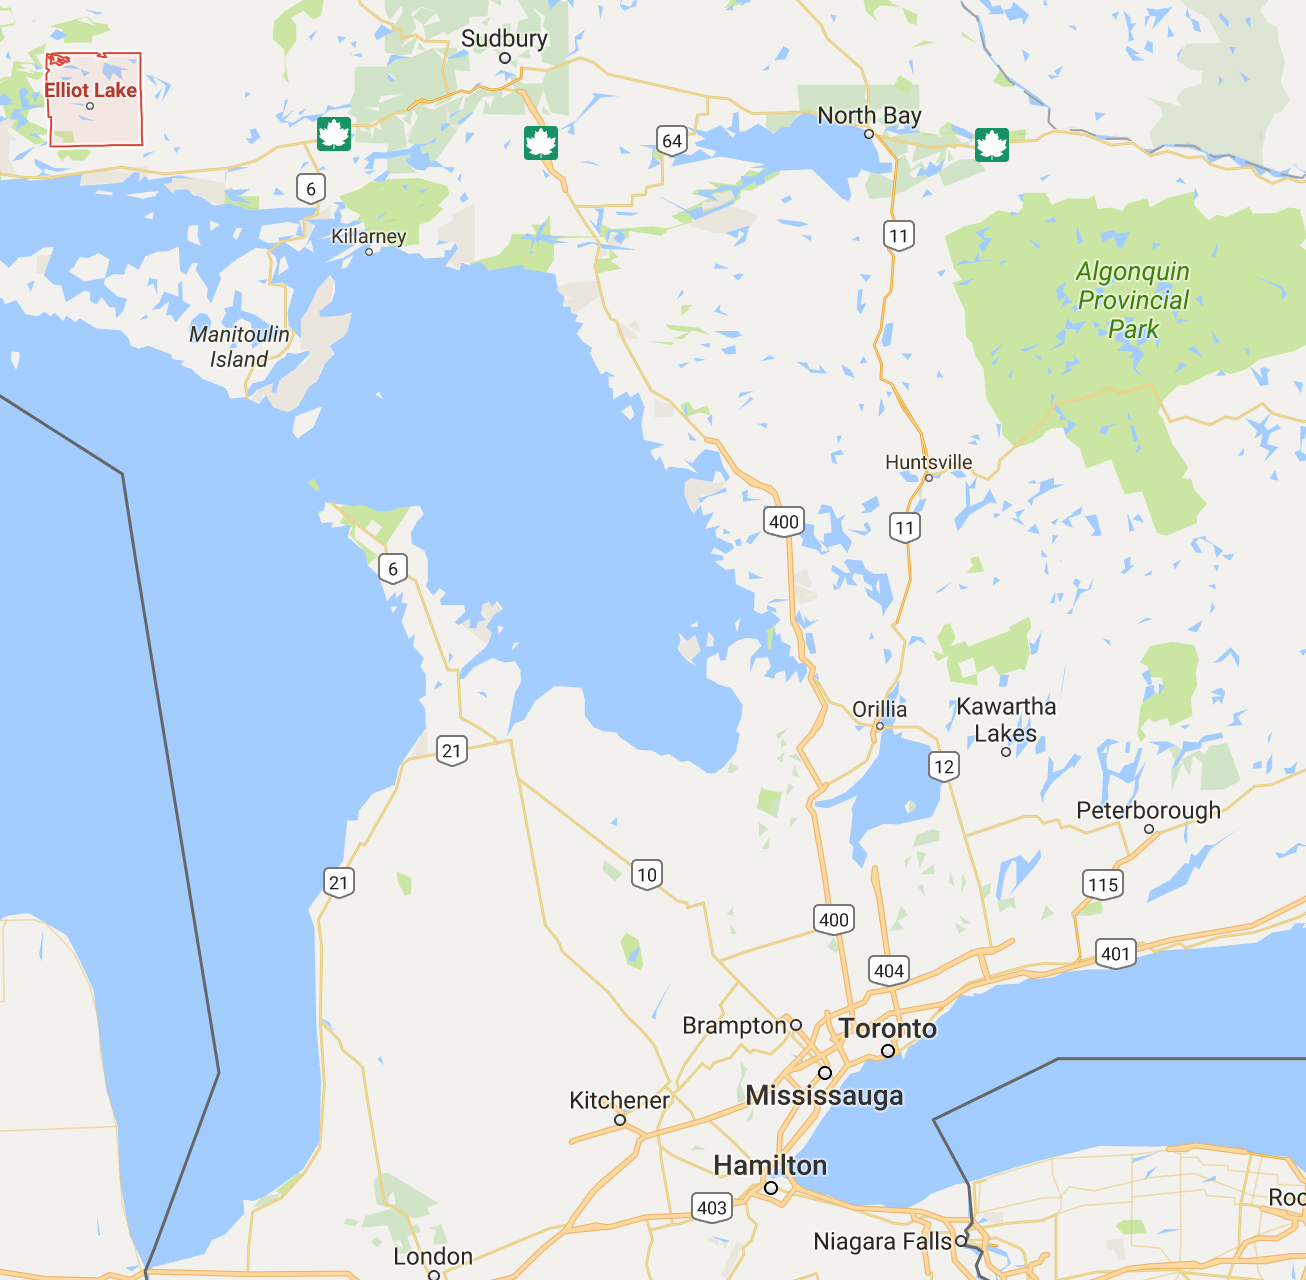
\includegraphics[width=0.65\textwidth]{images/Elliot-Lake-Map.png}
\end{center}
Source: Google Maps

\end{frame}



\begin{frame}
\frametitle{Algo Mall}

The mall was more than just a shopping centre. It was the town centre.

In addition to the usual stores, the mall also had federal and provincial offices, a library, and the offices of the area's MP and MPP.

The mall was built in 1979 and had apparently always had leakage problems, leading to jokes about ``Algo Falls''.

These warning signs were there but they were often ignored... 

\end{frame}



\begin{frame}
\frametitle{Human Failure}

Although rust was the proximate (immediate) cause of the collapse, the real failure was the human failure. 

To quote from the report~\cite{eli}:

\begin{quote}
Many of those whose calling or occupation touched the Mall displayed failings  --  its designers and builders, its owners, some architects and engineers, as well as the municipal and provincial offcials charged with the duty of protecting the public. Some of these failings were minor; some were not. They ranged from apathy, neglect, and indifference through mediocrity, ineptitude, and incompetence to outright greed, obfuscation, and duplicity. Occasional voices of alarm blew by deaf and callous ears. Warning signs went unseen by eyes likely averted for fear of jeopardizing the continuing existence of the Mall  --  the social and economic
hub in Elliot Lake.
\end{quote}


\end{frame}



\begin{frame}
\frametitle{This was Preventable}

The conclusions of the report, summarized are:
\begin{itemize}
	\item The collapse was due to a sudden failure of a connection between a beam and column of the steel substructure.
	\item This occurred because of ingress of water and chlorides (salt) from the deck of the mall which resulted in severe corrosion.
	\item The entry of water was caused by faulty design combined with inadequate and incompetent maintenance.
	\item There were many complaints, but these were often ignored.
	\item The situation was not taken seriously. 
	\item Some structural engineers failed to inspect the mall properly.
	\item Owners chose cheap \& ineffective repairs and attempted to conceal the problems.
\end{itemize}


\end{frame}



\begin{frame}
\frametitle{Observing the Collapse}

\begin{center}
\url{https://www.youtube.com/watch?v=PuckU1s5_gw}
\end{center}

\end{frame}



\begin{frame}
\frametitle{Professional Involvement}

In 1979, Algocen Realty Holdings constructed the centre and it was built with steel beams combined with precast hollow core concrete slabs.

The mall's roof was an unsheltered 334-space parking lot.

The structural design was signed and stamped by a Professional Engineer. 

Algocen received warnings about the potential for the roof to leak.

The warnings were ignored due to cost and land availability.

\end{frame}



\begin{frame}
\frametitle{Professional Non-Involvement}

No individual was responsible for the entire construction.

The architect merely prepared the drawings; the engineer handled the design; a Michigan company designed and applied the waterproofing system.

In spite of their limited knowledge, the architect and engineer signed \& sealed a document to the town saying the building was substantially complete.

\end{frame}



\begin{frame}
\frametitle{Fault of the Owners \& City}

Much fault can be laid at the feet of three owners, all of whom could easily have afforded to repair the problem, but did not do so.

The report examines in some detail the deception of the owners and how they pretended to care but never wanted to actually go through with it.

Similarly, the city was aware of the problem but made limited efforts to do anything about it and did not pursue the issue.

But we're mostly interested in the actions of the engineering professionals...

\end{frame}



\begin{frame}
\frametitle{2009 ``Inspections''}

The mall was inspected by professionals twice in 2009.\\
\quad Inspectors failed to grasp the serious of the situation.

In May 2009 an engineer and certified engineering technologist did a building condition assessment... badly.

The company did not look at its own past reports before the inspection, nor did they get other engineering reports that explained the true nature of the leaks.

The inspection was a visual assessment when it had not recently rained.\\
\quad None of the tenants were asked about the subject.\\
\quad Only two openly visible areas of the mall's structure were examined.

In spite of the dangerous situation, the report said: condition ``satisfactory''.


\end{frame}



\begin{frame}
\frametitle{2009 ``Inspections''}

There was a 2006 Notice of Violation ignored for some three years.

The city's fire chief managed to convince the chief building official to take a look.

He discovered water infiltration, abundant rust, and missing or waterlogged fireproofing on the steel beams.

The city issued an order for another inspection. An engineer was retained...\\
\quad Robert Wood, P.Eng. had been practicing since 1974. 35 years!

\end{frame}



\begin{frame}
\frametitle{Where To Begin...}

The commission report found the inspection, let's say, ``seriously deficient''!

How did Mr. Wood do this inspection badly?
\begin{itemize}
	\item He was provided with a 1998 report which he did not read.
	\item He limited his work to only specific areas of leakage despite being ordered to inspect the entire mall.
	\item He did not assess the waterproofing system even though the order said so.
	\item He was not provided with the 2006 Notice of Violation, the extent of previous leaks, other engineering reports.
	\item He spent less than one day at the mall with only a tape measure, flashlight, and notepad.
	\item He did not look at past report by the company about the mall which indicated the leaks had corned for some 16 years.
	\item He inspected the beam that eventually collapsed and photographed it, but did not look at the connections.
	\item He dismissed the concerns of the mall employees about vibrations.
\end{itemize}

\end{frame}



\begin{frame}
\frametitle{And the Report, Too}

The report produced after this inspection was similarly deficient.

\begin{itemize}
	\item The report did not provide a plan to correct deficiencies.
	\item The report in fact said he did not find any structural concerns, despite not having taken detailed measurements.
	\item No consequences were enumerated if the leaks were to continue.
\end{itemize}

\end{frame}



\begin{frame}
\frametitle{The Ministry Did It Wrong Too}

In January 2012 the ministry did another inspection and it was also inadequate.

The inspection was very brief, and he did not notice leaks, buckets, tarps...\\
\quad But he did not speak to tenants, employees, etc...

\end{frame}



\begin{frame}
\frametitle{It Gets Worse!}

Mr. Wood was asked to do another inspection in April 2012.

Mr. Wood conducted the inspection while his license was suspended.\\
\quad He was required to have a P. Eng. review his work.

He took on the mall owners as a client even though he was asked by his firm not to take on any new clients.

The commission found Mr. Wood did not conduct the inspection objectively...\\
\quad He had a preconceived notion that the mall was structurally sound.

Mr. Wood's partner, Gregory Saunders, P.Eng., was asked to review the report.\\
\quad After about 45 minutes, Mr. Saunders signed the report.

\end{frame}



\begin{frame}
\frametitle{Careful Review... It Is Not}

Mr. Saunders did not know about the Order to remedy, the previous report, or the history of leaks at the mall.

Mr. Saunders had never been to the mall and did no investigations of his own.\\
\quad Given Wood's suspension, Saunders really should have been more critical...

Following the meeting, Mr. Wood made changes to the report without advising Saunders, and this was more favourable to the owners.

\end{frame}



\begin{frame}
\frametitle{Report Recommendations}

The report contained, in particular, one recommendation for PEO:

The Professional Engineers of Ontario should establish a system of mandatory continuing professional education for its members as soon as possible, and in any event no later than 18 months from the release of this Report.

\end{frame}



\begin{frame}
\frametitle{PEO Task Force}

PEO created a task for preparing a response to this recommendation.

The Task Force has developed a framework for a proposed CPD program that:

\begin{enumerate}[i)]
	\item Recognizes there are practicing and non-practicing license holders.
	\item Focuses on maintaining provision of competent engineering services rather than introducing a bureaucratic hurdle.
	\item ensures CPD requirements will be based on the risk that the work of the individual licence holder presents to the public and the profession.
	\item encourages licence holders and their employers to adopt risk mitigation measures within the work environment.
	\item improves on programs implemented by associations in other provinces.
\end{enumerate}

The report can be read at \url{http://peo.on.ca/index.php/ci_id/29313}.

\end{frame}



\begin{frame}
\frametitle{Guiding Principles}

Quoting from the report:

1. \textbf{CPD Program must be necessary to improve the regulation of professional engineering.}

Those advocating for a CPD program often point out that PEO is the only professional engineering association in Canada that does not have CPD. 

The Task Force felt that no program should be put in place solely for PEO to say they have a program.

\end{frame}



\begin{frame}
\frametitle{Guiding Principles}

Quoting from the report:

2. \textbf{CPD Program Requirements must be Relevant for Practice}


Whatever CPD program is established it must be relevant to the practice of professional engineering.

It must be done in the interest of safeguarding public health, safety and welfare. 


\end{frame}


\begin{frame}
\frametitle{Guiding Principles}

Quoting from the report:

3. \textbf{CPD Program must be Pragmatic}

The purpose of any future PEO CPD program should be to ensure that practitioners maintain a level of knowledge and skill commensurate with safeguarding the public


\end{frame}

\begin{frame}
\frametitle{Guiding Principles}

Quoting from the report:

4. \textbf{CPD Program must recognize Diversity of Practitioners' needs/resources}

PEO should not rely on a one size fits all CPD approach as in other provinces. 

A single all-encompassing CPD program would be either too onerous for some licence holders or watered-down to meaninglessness for others. 

\end{frame}



\begin{frame}
\frametitle{Guiding Principles}

Quoting from the report:


5. \textbf{CPD Program Requirements must be Scalable and Proportional to Risk to the Public}

The Task Force decided to address the diversity of practice among licence holders by adopting a risk-based approach to CPD. 

That is, CPD requirements would be correlated to the amount of risk to the public the practitioner's work entails. 

\end{frame}




\begin{frame}
\frametitle{Suggested Review Parameters}

The task force suggests some criteria for evaluation of risk:

\begin{enumerate}
	\item Area of practice
	\item External industry certification requiring CPD
	\item Percentage of time practicing
	\item Scope of practice recently changed?
	\item Emerging field of technology
	\item Level of responsibility in the organization
	\item Severity of errors or omissions in work done
	\item Severity of consequences due to practitioner error
	\item Professional liability insurance?
	\item Well-established industrial codes \& standards?
	\item Firm audited by industry QA program?
	\item Size and structure of organization
	\item Internal QA processes and peer reviews
\end{enumerate} 


\end{frame}



\begin{frame}
\frametitle{Guiding Principles}

Quoting from the report: 

6. \textbf{CPD Program must be Effective}

There must be a means for determining whether the program is effective.

PEO must have a system to ensure that members who consider their work to be low risk are not actually doing high risk work. 

For instance, control and software engineers have reported that they have very little or no impact on the public safety. 

This may be the result of a misunderstanding of who the public is. 

The public includes workers in the plant and the firms and consumers to whom completed products are distributed.

... or what kinds of risks professional engineers are responsible for preventing or
mitigating.

\end{frame}



\begin{frame}
\frametitle{Consultations}

In late 2015 PEO held consultation town hall meetings in five chapter regions.

Consultations are ongoing and the program is still in development.

It is not clear what the final form of the CPD requirements will be, but the draft provides a pretty good indication of what will happen...


\end{frame}

\begin{frame}
\frametitle{References \& Disclaimer}
\bibliographystyle{alphaurl}
\setbeamertemplate{bibliography item}{\insertbiblabel}
{\scriptsize
\bibliography{290}
}
\vfill

{\tiny Disclaimer: the material presented in these lectures slides is intended for use in the course ECE~290 at the University of Waterloo and should not be relied upon as legal advice. Any reliance on these course slides by any party for any other purpose are the responsibility of such parties.  The author(s) accept(s) no responsibility for damages, if any, suffered by any party as a result of decisions made or actions based on these course slides for any other purpose than that for which it was intended.\par}


\end{frame}


\end{document}

